%------------------------------------------%
% Cannabis Data Science
% Date: 12/22/2021
%------------------------------------------%
\documentclass[xcolor={dvipsnames}]{beamer}
\hypersetup{pdfpagemode=FullScreen}
\mode<presentation>{
  \usetheme{Boadilla}
  \usecolortheme{orchid}
  \usefonttheme{default}
  \setbeamertemplate{navigation symbols}{}
  \setbeamertemplate{caption}[numbered]
} 
\usepackage[english]{babel}
\usepackage[utf8x]{inputenc}
\setbeamersize{text margin left=0.5in,text margin right=0.5in}

\usepackage[dvipsnames]{xcolor}
\definecolor{DarkGreen}{RGB}{2, 48, 32}
\definecolor{CalyxGreen}{RGB}{34, 153, 84}
\definecolor{DarkOrange}{RGB}{199, 0, 57}
\definecolor{LightOrange}{RGB}{255, 87, 51}
\definecolor{LightGreen}{RGB}{218, 247, 166}
\definecolor{LightYellow}{RGB}{255, 195, 0}

\setbeamercolor*{palette primary}{bg=LightGreen, fg = DarkGreen}
\setbeamercolor*{palette secondary}{bg=LightGreen, fg=DarkGreen}
\setbeamercolor*{palette tertiary}{bg=LightGreen, fg = DarkGreen}
%\setbeamercolor*{palette quaternary}{bg=myNewColorD, fg = green}

%------------------------------------------%
% Packages
%------------------------------------------%
\usepackage{amsmath}
\renewcommand*\footnoterule{} %No sperating line on footnote
\usepackage{mathtools} %ANNOTATING EQUATIONS
\usepackage{hhline} %DOUBLBARS
\usepackage[super]{nth}
\usepackage{graphicx, caption, subcaption}

%------------------------------------------%
% Commands
%------------------------------------------%
\newcommand\T{\rule{0pt}{2.5ex}} %TOPSTRUT
\newcommand\B{\rule[-1.25ex]{0pt}{0pt}} %BOTTOMSTRUT
\newenvironment<>{varblock}[2][.9\textwidth] %RESIZED BLOCKS
  {\setlength{\textwidth}{#1}
  \begin{actionenv}#3
    \def\insertblocktitle{#2}\par
    \usebeamertemplate{block begin}}
  {\par\usebeamertemplate{block end}
  \end{actionenv}}
\defbeamertemplate{enumerate item}{largeball} %LARGE BALLS
{\begin{pgfpicture}{-1ex}{-0.65ex}{1.5ex}{1.5ex}
\usebeamercolor[fg]{item projected}
{\pgftransformscale{2.5}\pgftext{\Large\pgfuseshading{bigsphere}}}
{\pgftransformshift{\pgfpoint{0pt}{0.5pt}}
\pgftext{\usebeamerfont*{item projected}\small\insertenumlabel}}
\end{pgfpicture}}
\usepackage{tikz} % FANCY ARROWS
\usepackage{xparse}
\NewDocumentCommand\UpArrow{O{2.0ex} O{black}}{%
   \mathrel{\tikz[baseline] \draw [->, line width=0.5pt, #2] (0,0) -- ++(0,#1);}} % FANCY UPARROW
\NewDocumentCommand\DownArrow{O{2.0ex} O{black}}{%
   \mathrel{\tikz[baseline] \draw [<-, line width=0.5pt, #2] (0,0) -- ++(0,#1);}} % FANCY DOWNARROW
%\vskip 1cm
\makeatletter
\newcommand{\LeftEqNo}{\let\veqno\@@leqno}%LEFT EQUATION #'s
\makeatother

%------------------------------------------%
% Title
%------------------------------------------%
\title[\textbf{Meetup}]{}
\author{Cannabis Data Science}
\institute[]{\Large Meetup}
\date{December \nth{22}, 2021}
\begin{document}
\begin{frame}{}
  
\includegraphics[scale=0.075]{images/logos/cannlytics_logo_with_text_light.png}
  \titlepage
\end{frame}

%------------------------------------------%
% Introduction
%------------------------------------------%

\section{Introduction}

%------------------------------------------%
% State Data
%------------------------------------------%

\begin{frame}{}

{\large \textbf{Research Question}: What is the relationship between dispensaries per capita and revenue per dispensary?}\vspace{0.5\baselineskip}\\

\begin{figure}
    \begin{subfigure}[t]{\textwidth}
      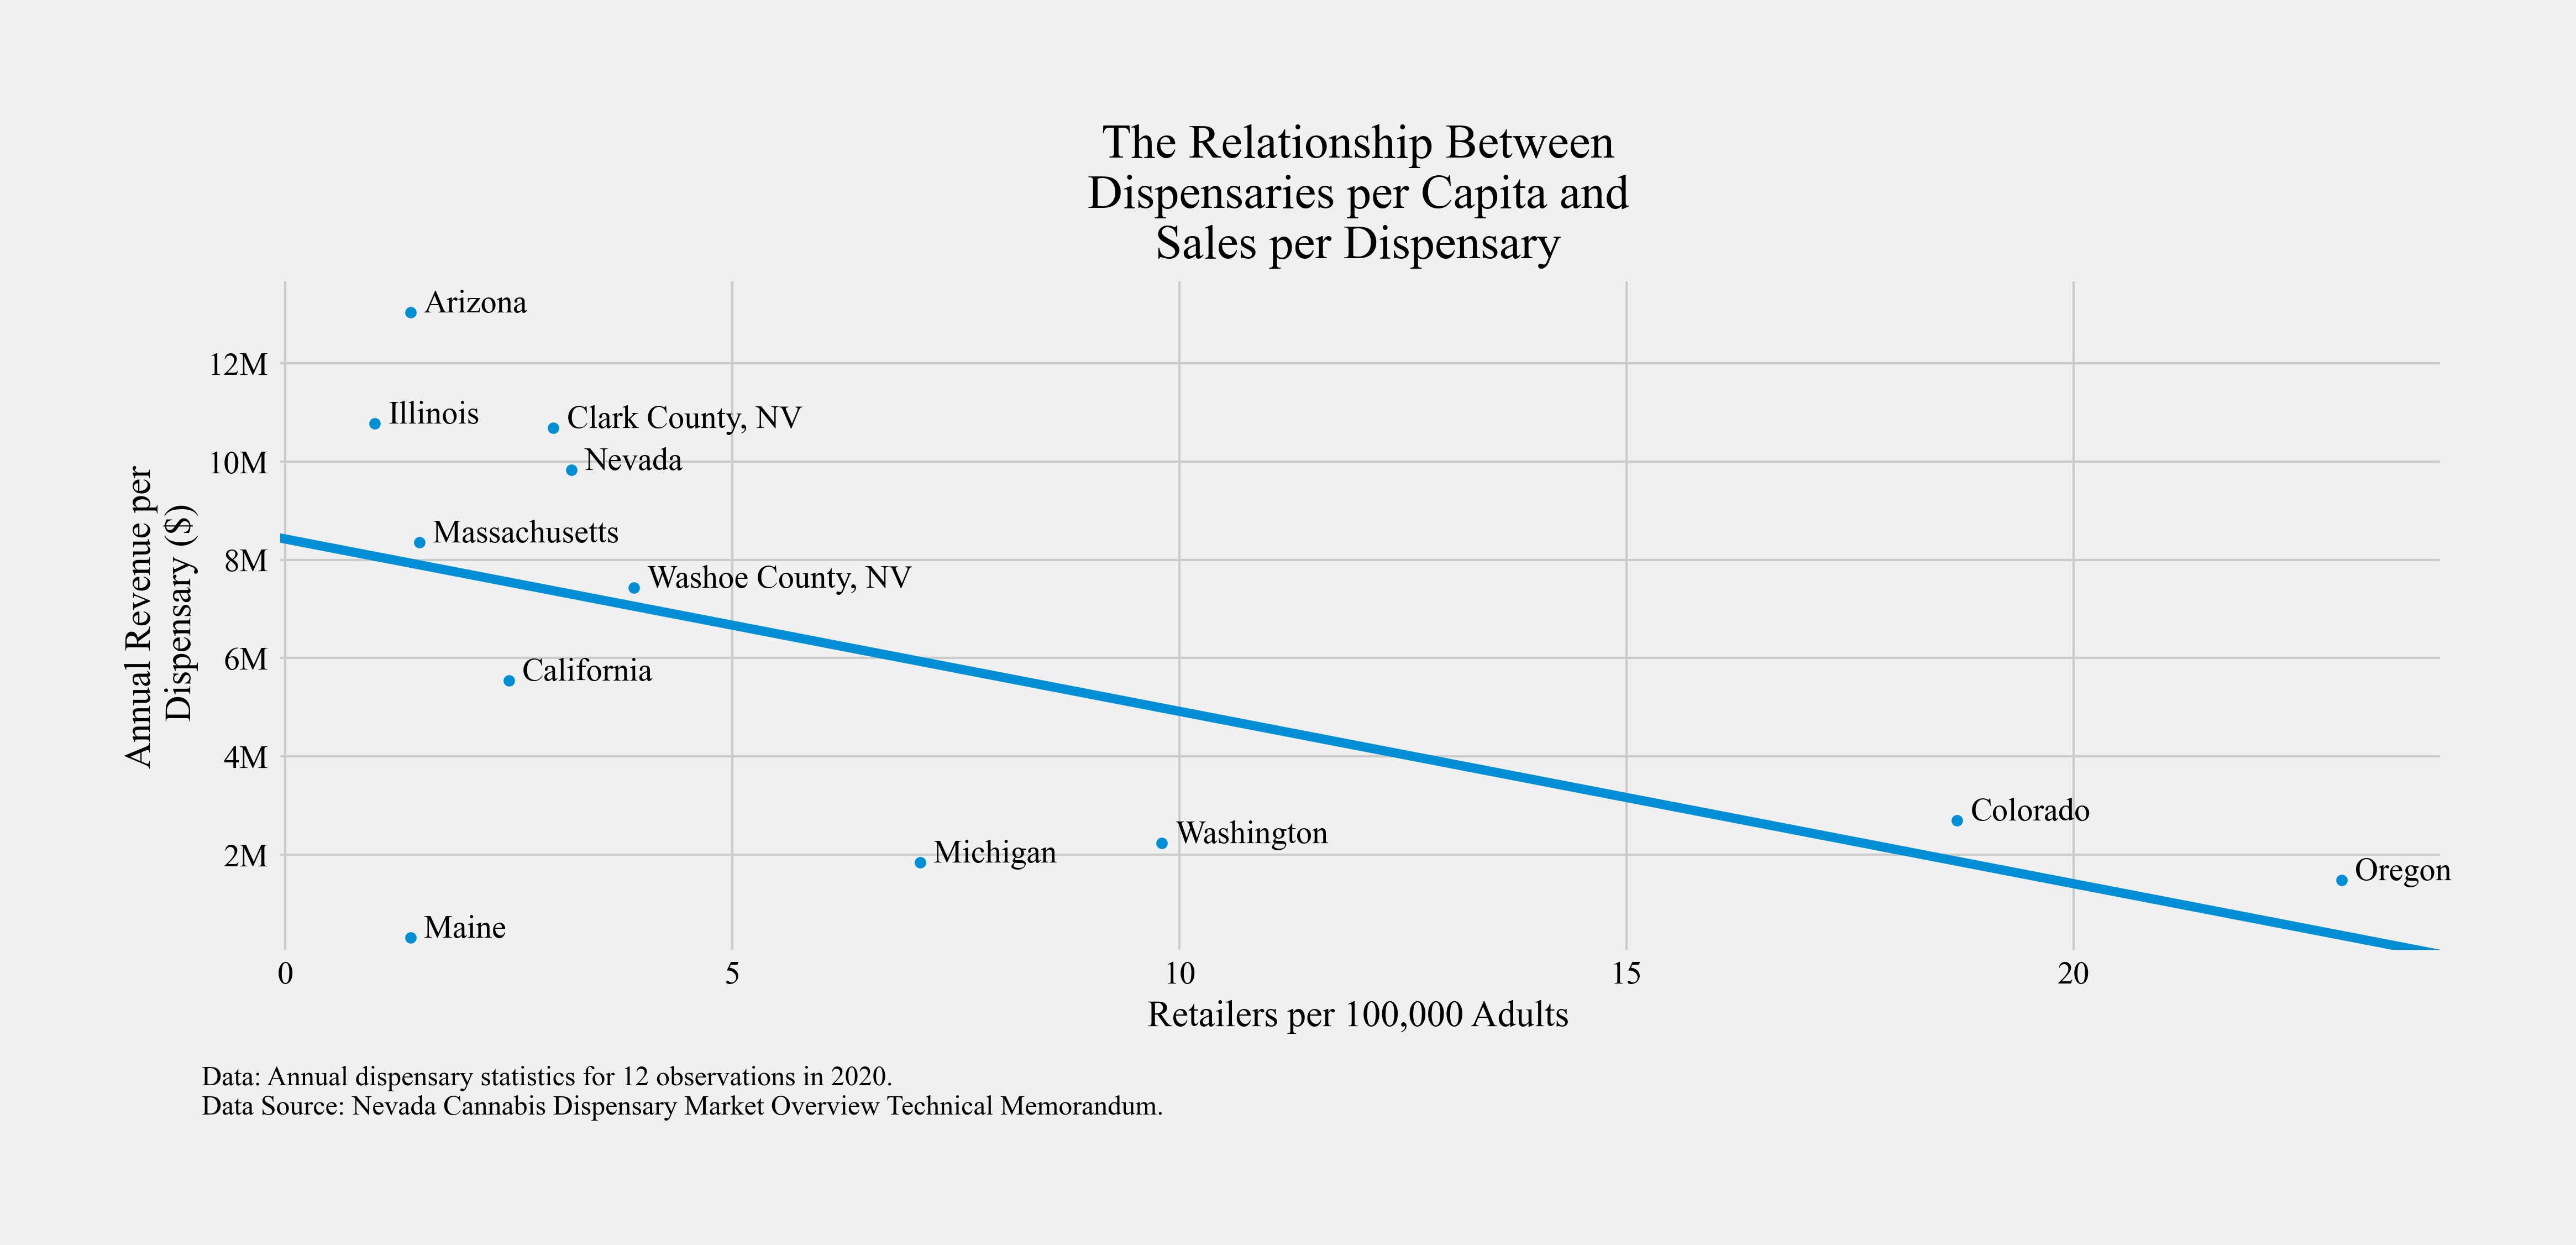
\includegraphics[width=\textwidth]{images/revenue_per_retailer_to_retailers_per_100_000.png}
    \end{subfigure}
\end{figure}


\end{frame}

%------------------------------------------%
% Forecasting
%------------------------------------------%

\begin{frame}{}

{\large \textbf{The 10 Commandments of Forecasting}}
\vspace{1\baselineskip}

{\scriptsize Silvia, J, Iqbal, A, et. al (2014), ‘Economic and Business Forecasting’.}

\vspace{1\baselineskip}

\begin{enumerate}
\item Know what you are forecasting.
\item Understand the purpose of forecasting.
\item Acknowledge the cost of the forecast error.
\item Rationalize the forecast horizon.
\item Understand the choice of variables.
\item Rationalize the forecasting model used.
\item Know how to present the results.
\item Know how to decipher the forecast results.
\item Use recursive methods.
\item Understand that forecasting models evolve over time.
\end{enumerate}
\end{frame}

%------------------------------------------%
% RMSE
%------------------------------------------%

\begin{frame}{}

{\large \textbf{Measuring Forecast Error}}\vspace{0.5\baselineskip}\\

The out-of-sample root mean square error (RMSE) can quantify forecast error.

$$
RMSE = \sqrt{\frac{1}{T}\Sigma(Y_{t+1} - \hat{Y}_{t+1})^2}
$$
\end{frame}

%------------------------------------------%
% Panel Data
%------------------------------------------%
\section{Panel Data}

\begin{frame}{}

{\large \textbf{Panel Data}}\vspace{0.5\baselineskip}\\

A panel has the form

\begin{figure}
    \begin{subfigure}[t]{.5\textwidth}
      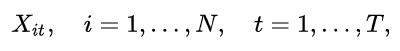
\includegraphics[width=\textwidth]{images/panel.png}
    \end{subfigure}
\end{figure}

where $i$ is the individual dimension and $t$ is the time dimension.\vspace{0.5\baselineskip}\\

A general panel data regression model is written as

\begin{figure}
    \begin{subfigure}[t]{.3\textwidth}
      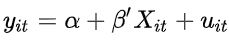
\includegraphics[width=\textwidth]{images/regression.png}
    \end{subfigure}
\end{figure}

where

\begin{figure}
    \begin{subfigure}[t]{.25\textwidth}
      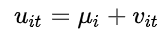
\includegraphics[width=\textwidth]{images/errors.png}
    \end{subfigure}
\end{figure}

Estimation with a \textbf{fixed effects} or \textbf{random effects} model depends on assumptions about $\mu_i$, the individual-specific, time-invariant effects.

\end{frame}

%------------------------------------------%
% Takeaway
%------------------------------------------%

\begin{frame}{}

\begin{center}
\begin{minipage}{3.85in}


\includegraphics[width=.25in]{images/prayer.png} {\Large \textbf{Thank you for coming.}}\vspace{0.5\baselineskip}\\

Take some time, discuss any conclusions drawn, and try to make some forecasts of your own!

\end{minipage}
\end{center}

\end{frame}

%------------------------------------------%
% Finale
%------------------------------------------%
\end{document}
